\documentclass[11pt,a4paper,titlepage]{report}
\usepackage[latin1]{inputenc}
\usepackage{amsmath}
\usepackage{amsfonts}
\usepackage{amssymb}
\usepackage{graphicx}
\usepackage[section]{placeins}
\usepackage{float}
\usepackage{url}
\usepackage[font=small]{caption}
\providecommand{\tightlist}{%
	\setlength{\itemsep}{0pt}\setlength{\parskip}{0pt}}

% todo notes
\usepackage[colorinlistoftodos,prependcaption,textsize=tiny]{todonotes}

\author{MERMET Alexis}
\title{Bachelor Project: Augmenting \textit{pyroomacoustics} with machine learning utilities}
\date{June 8, 2018}

\begin{document}
\maketitle
\tableofcontents
\newpage
%...
\chapter{Introduction}
\section{Objectives of the project}
\hspace*{0.6cm}

\todo{can you look into using bibtex? so that you can cite reference directly in the paper.}

During this project, we want to implement new functionalities to the already existing Python library, \textit{pyroomacoustics}\todo{change mentions of \textit{pyroomacoustics} to this style and check for typos!}. These functionalities include a wrapper to Google's Speech Commands Dataset\todo{add reference here}, utilities for augmenting  datasets with the already-available room impulse response (RIR) generator, and scripts for evaluating the performance of single and multi-microphone processing for speaker recognition against a pre-trained model. 

\section{What is \textit{pyroomacoustics}?}

\hspace*{0.6cm}
First of all Pyroomacoustics is a library allowing us to make audio room simulation  and also apply array processing algorithm in Python. Developed by former and current EPFL undergraduate and graduate students, the goal of this library is to aid in ``the rapid development and testing of audio array processing algorithms.'' There are three core components:
\begin{enumerate}
	\tightlist
	\item Object-oriented interface in Python for constructing 2D and 3D simulation scenarios;
	\item A fast C implementation of the image source model for room impulse response (RIR) generation;
	\item Reference implementations of popular algorithms for beamforming, direction finding, and adaptive filtering.
\end{enumerate} 
\hspace*{0.6cm} 
Before the start of this project, we could find three main classes\todo{there's at least two more for DOA and adaptive filtering} in Pyroomacoustic: The Room class, the SoundSource class and the MicrophoneArray class. Quickly after I began working, Robin Schleiber also added a Dataset class that helped me to start creating a wrapper for Google's Speech Commands Dataset (explained below).\\
\\
\hspace{0.6cm}
With the Room class, you create an object that is a collection of Wall objects, a MicrophoneArray and a list of SoundSource(s). It can be either 2D or 3D.
A SoundSource object has as attributes the location of the source itself and also all of its images sources. In general we create this list directly in the Room object that contains the source.
Finally the MicrophoneArray class consist of an array of microphone locations together with a sampling frequency.
\begin{figure}[h!]
	\centering
	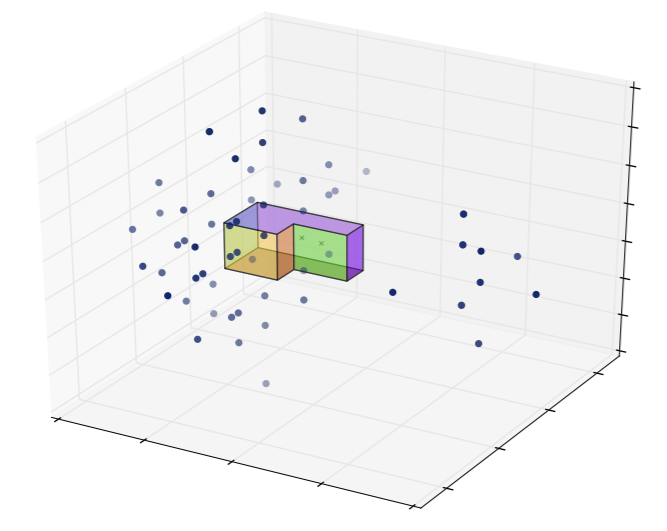
\includegraphics[width=0.7\linewidth]{rapport1}
	\caption[Example of a room in Pyroomacoustic]{Example of a room in Pyroomacoustic.}
\end{figure}

\section{What is Tensorflow?}
\hspace*{0.6cm}
\todo{references!}
As they say on their website, Tensorflow is an "open source software library for high performance numerical computation". We followed a Tensorflow tutorial called "Simple Audio Recognition" to create the neural networks we used during the all project (we are going to explain how it was created in 2.1). We have also reimplemented some of their functions to be able to label sounds we have modified through processing (see~\ref{sec:label_file}).\todo{you can make links between section, images, etc with the ``label'' and ``ref'' tags}
\chapter{Theoretical knowledge}
\section{Training the Neural Network}
\hspace*{0.6cm}
In this section we're going to talk about how the neural network was trained. First off all, we download the GoogleSpeechCommand\todo{this is not the official name so I would change to referring it as ``Google's Speech Commands dataset''. ``GoogleSpeechCommand'' is the name we use for our wrapper} dataset since we need it to train our network but to test the efficiency of our algorithms. According to the tutorial, this model is considered really simple but is also ``quick to train and easy to understand".\\
\hspace*{0.6cm}
This model works as a convolutional network (in fact this model is similar to the one you can use to do some image recognition). First of all a window of time is defined and the audio signal is converted to an image with the Short Time Fourier Transform (STFT), i.e.\ a spectrogram. This is done by \todo{change beginning quotes to ``}"grouping the incoming audio samples into short segments and calculating the strength of the frequencies across a set of bands". All the frequency strengths of a given segment will then be treated as a vector of values. These vectors are then ordered according to the time, forming the two-dimensional array known as a ``spectrogram''\\
\begin{figure}[h]
	\centering
	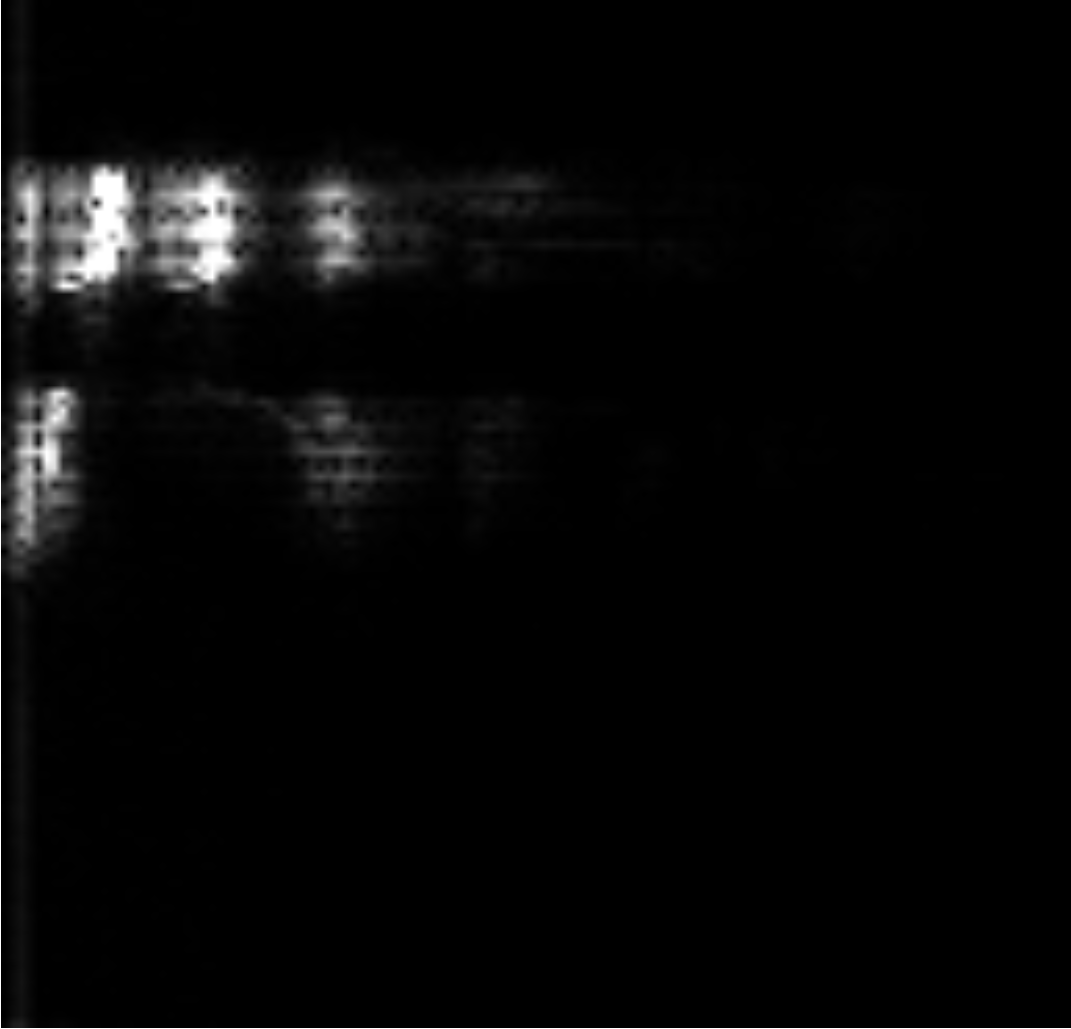
\includegraphics[width=0.7\linewidth]{Rapport2}
	\caption{Spectrogram of one of our sample during the training (image of the Tensorflow website).}
\end{figure}

\hspace*{0.6cm}
In the figure 2.1, time is increasing from top to bottom and frequencies from left to right. We can also different part of the sound that are probably specific part of it (like a syllable in our case of word).\todo{this last sentence is unclear...}\\
\hspace*{0.6cm}
After our ``image'' is created we can feed it into a multi-layer convolutional neural network (CNN), with a fully-connected layer followed by a softmax at the end. With a large amount of images and associated labels, we can train our network to classify different words. It took between 16h-20h to train the model and we're going to look at its accuracy later on in this report.


\section{The GoogleSpeechCommands Dataset: Basic informations}
\hspace*{0.6cm}
Created by the \todo{be consistent with how you mention TensorFlow}tensorflow and AIY teams, the speech command dataset is used to add training and inference in tensorflow. The dataset contains 65,000 one-second long sound of 30 short words, spoke by "thousands of different people". This dataset is not fixed and will continue to increase with the contribution of users. It is designed to help a user to create his own basic voice recognition interface, with common words like `yes', `no', directions, etc...\\


\begin{figure}
	\centering
	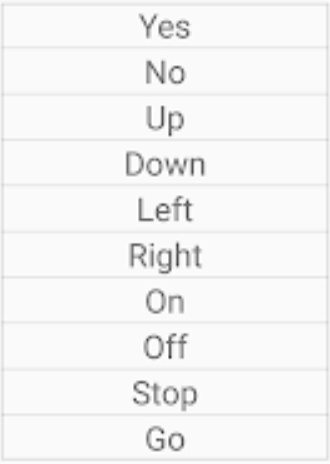
\includegraphics[width=0.4\linewidth]{rapport3}
	\caption{The different words our system is able to recognize}
\end{figure}
\todo{Figure 2.2 is bit blurry, perhaps you can list the words separately}

\section{Some Signal Processing concepts}
\hspace*{0.6cm}
In this section we're going to talk about one of the most important concept of signal processing we used during this project: the Signal to Noise Ratio (SNR) and everything that comes from it. Even though this concept is quite simple and well known, we will talk about it cause we used it nearly everywhere as you'll see later when we will talk about the implementation (Chapter 4).\\
\hspace*{0.6cm}
First of all, for a single sensor, considering the signal y(t) = s(t) + n(t), with s(t) being the sound of interest and n(t) being the noise, the Signal to Noise Ratio is defined as the sound power over the noise power.
\[SNR\textsubscript{sensor} = \dfrac{E[|s(t)^2|]}{E[|n(t)^2|]} = \dfrac{\sigma\textsubscript{s}^2}{\sigma\textsubscript{n}^2}  \] 
with $\sigma\textsubscript{s}^2$ being the power of the sound of interest and $\sigma\textsubscript{n}^2$ being the power of the noise.\\
Then if we know consider an array of M sensors and define that the signal received at the sensor m is y\textsubscript{m}(t) = s\textsubscript{m}(t) + n\textsubscript{m}(t). We define the signal for the all array Z(t) such that:
\[Z(t) = \sum_{m=0}^{M-1}{w\textsubscript{m}* y\textsubscript{m}(t-\Delta\textsubscript{m})} = Z\textsubscript{s}(t) + Z\textsubscript{n}(t) \]
with w\textsubscript{m} being the weight corresponding to the signal y\textsubscript{m} and $\Delta$\textsubscript{m} being a delay that represents the fact that the sound doesn't arrive at the same moment to each sensor.\\
Now we can write that the SNR value of our signal Z(t) is:
\[SNR\textsubscript{array} = \dfrac{E[|Z\textsubscript{s}(t)^2|]}{E[|Z\textsubscript{n}(t)^2|]} = \dfrac{|\sum_{m}w\textsubscript{m}|^2*\sigma\textsubscript{s}^2} {\sum_{m}|w\textsubscript{m}|^2*\sigma\textsubscript{n}^2} \] 
\hspace*{0.6cm}
Finally in this project we don't use the SNR under this form cause it is not really intelligible and easy to use. So we convert it into decibels (dB) such that we know have:
\[ SNR\textsubscript{dB} = 10\log\textsubscript{10}{\dfrac{\sigma\textsubscript{s}^2}{\sigma\textsubscript{n}^2}} \]

\section{The algorithms}
\hspace*{0.6cm}
In this section we are going to talk about the different algorithm we used in this project.
\subsection{Single Noise Channel Removal}
\hspace*{0.6cm}
The Single Noise Channel Removal is used to suppress the noise. We consider a noisy input signal x[n] that becomes X(k,i), once converted into the frequency domain using the STFT (Short Time Fourier Transform). The noise suppressor removes the noise by applying a time-frequency-varying real-valued gain filter G(k,i) to X(k,i). We define this gain filter has follow:\\
-When, at a given time and frequency, there is no noise, the gain filter has value 1.\\
-When, at a given time and frequency, there is only noise, the gain filter has value G\textsubscript{min}.
-When, at a given time and frequency, there is a mix of signal and noise, the gain filter has a value between G\textsubscript{min} and 1.\\
\hspace*{0.6cm}
For this algorithm, an estimation of the noise is needed, we have:
 \[P(k,i) = E[|X(k,i)|^2]  \]
and we need to compute a noise estimator, P\textsubscript{N}(k,i). There is two ways to compute it:\\
1) if the noise is stationary: P\textsubscript{N}(k,i) = min P(k,i) over time.\\
2) use a voice detector: P\textsubscript{N}(k,i) = P(k,i) during a silence period. \\
so: 
\[P\textsubscript{N}(k,i) = \min_{0 \eqslantless l \eqslantless k} P(k,i)\]
Now we can define our Gain filter such that:
\[ G(k,i) = \max[\frac{(P(k,i)- \beta*P\textsubscript{N}(k,i))^\alpha}{P(k,i)^\alpha}, G_{min}] \]
where $\beta$ is an overestimation factor, often set to a value larger than one to ensure all noise is suppressed by a factor of $G_{min}$, and the exponent $\alpha$ controls the ransition behaviour of the gain filter between $G_{min}$ and one.
\begin{figure}
	\centering
	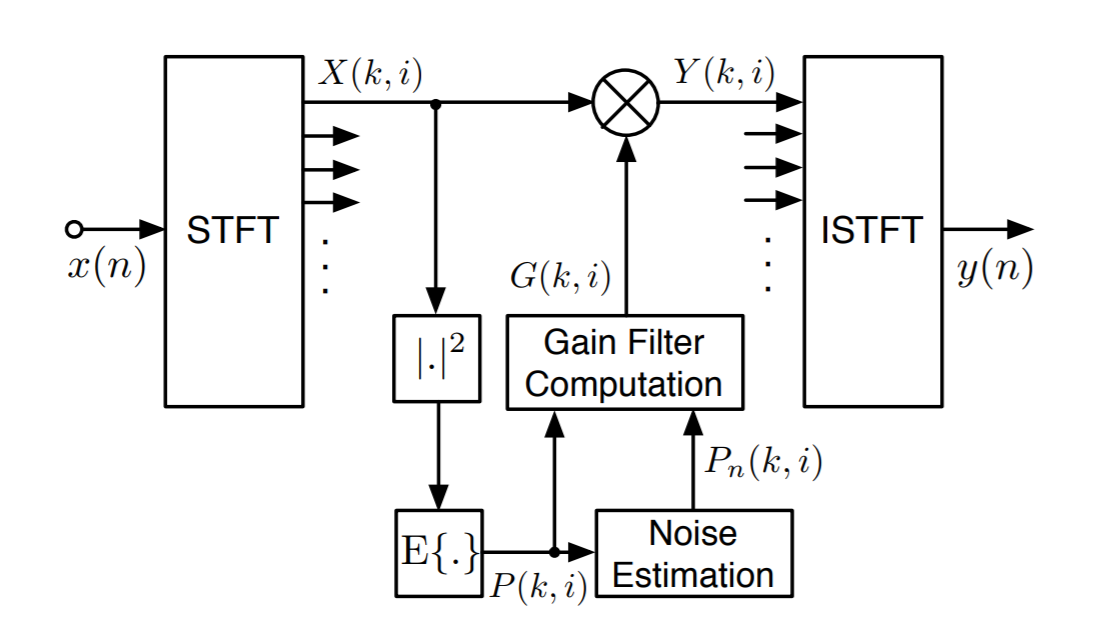
\includegraphics[width=0.7\linewidth]{rapport4}
	\caption{STFT-based stationary noise suppressor (from the Audio Signal Processing and Virtual Acoustics books).}
	\label{fig:rapport4}
\end{figure}

\subsection{Beamforming: Delay and Sum Weights}
\hspace*{0.6cm}
In this section we are going to talk about one of the easiest Beamforming algorithm. But first of all, the term Beamforming is used to talk about An ?intelligent? combination of the sensor signals to increase the SNR of the signal. Delay and Sum Weights also called Delay And Sum (DAS) is in fact what we have saw before hand in 2.3.\\
If we consider an array of M sensors and define that the signal received at the sensor m is $x_m(t)$ then we define Y(t) such that:
\[Y(t) = \sum_{m=0}^{M-1}{w\textsubscript{m}* x\textsubscript{m}(t-\Delta\textsubscript{m})}\]
with w\textsubscript{m} being the weight corresponding to the signal x\textsubscript{m} and $\Delta$\textsubscript{m} being a delay chosen to maximize the array's sensitivity to waves propagating from a particular direction.

\chapter{Implementation}
\section{The GoogleSpeechCommands Dataset}
\hspace*{0.6cm}
The "GoogleSpeechCommands" dataset wrapper was created has a subclass of the "Dataset" class that was already implemented in Pyroomacoustics. This class will load the Google Speech Commands Dataset in a structure that is convenient to be processed. It has four main attributes: the directory where the dataset is located, the "basedir". A dictionary whose keys are word in the dataset. The values are the number of occurrences for that particular word. It is called "sizebysamples". A list of subdirectories in "basedir", where each sound type is the name of a subdirectory, called "subdirs". And finally "classes",the list of all sounds, same as the keys of sizebysamples.\\
\\
\hspace*{0.6cm}
There are multiple functions in this class and we're going to review them quickly to give you a general idea of what is possible because of the model created in Pyroomacoustics.\\
\\
\hspace*{0.6cm}
1) we have the "init" function that is the builder of our class. When creating a structure containing the Google Speech Command dataset, the user can choose if he wants to download it or not. But he can also choose if he wants to construct just a subset of the all dataset at the start.\\
\begin{figure}[h!]
	\centering
	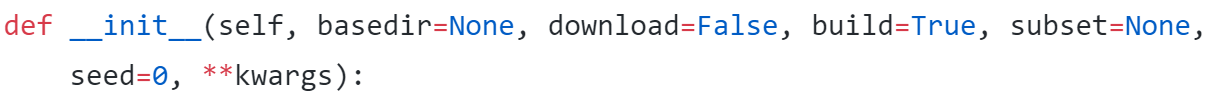
\includegraphics[width=0.95\linewidth]{Rapport5}
	\caption{The "init" function of a GoogleSpeechCommands structure}
	\label{fig:rapport5}
\end{figure}
\hspace*{0.6cm}
\\
2) The "build corpus" function that allows the user to build the corpus with some filters, as for example the list of the desired words to be taken from the corpus.\\
\begin{figure}[h!]
	\centering
	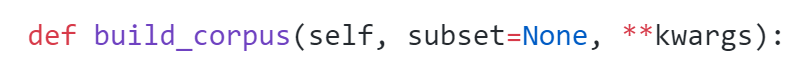
\includegraphics[width=0.7\linewidth]{Rapport6}
	\caption{The "build corpus" function from the wrapper}
	\label{fig:rapport6}
\end{figure}
\\
\hspace*{0.6cm}
3) The "filter" function that allows the user to filter the dataset and select samples that match the criterias provided.\\
\begin{figure}[h!]
	\centering
	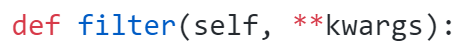
\includegraphics[width=0.4\linewidth]{Rapport7}
	\caption{The "filter" function from the wrapper}
	\label{fig:rapport7}
\end{figure}
\\
\hspace*{0.6cm}
Now that we talk about the wrapper, we need to present also the "GoogleSample" class that is inheriting from the class "AudioSample" created beforehand in Pyroomacoustics. This class allows the user to create an audio object to print it in a nice way and also to plot the corresponding spectrogram. 

\section{How to label a file?}
\label{sec:label_file}
\section{How to synthesize noisy signals}
\section{The algorithms}
\chapter{Results}
\section{Analyse improvement of Single Noise Channel Removal}
\section{Analyse improvement of Beamforming}
\chapter{Conclusion}
\section{Where are we now?}
\section{What's next?}
\chapter{Bibliography}
1) arXiv:1710.04196v1 [cs.SD],
	Robin Scheibler, Eric Bezzam,
		Ivan Dokmanic, \textit{"Pyroomacoustics: a python package for audio room simulation and array processing algorithms"},
	Ecole Polytechnique F�d�rale de Lausanne (EPFL),
		University of Illinois Urbana-Champaign, USA,
	11 Oct 2017
\\
\\
2) Tensorflow,
	\textit{Simple Audio Recognition},
	13 January 2018,
	\url{https://www.tensorflow.org/versions/master/tutorials/audio_recognition}
\\
\\
3) Pete Warden, Software Engineer, Google Brain Team, 
   Google AI Blog,
   \textit{Launching the Speech Command Dataset}
   24 August 2017
   \url{https://ai.googleblog.com/2017/08/launching-speech-commands-dataset.html}
\\
\\
4) J�rgen Grythe, 
	\textit{Array gain and reduction of self-noise}, 
	Norsonic AS, Oslo, Norway,
	2016
\\
\\
5) Christof Faller and Dirk Schr�der,
	\textit{Audio Signal Processing and Virtual Acoustics},
	9 September 2015,
\\
\\
6) 10.1109/ICASSP.2015.7178030,
	Robin Scheibler, Ivan Dokmanic, and Martin Vetterli, 
	\textit{Raking Echoes in the time domain }, 
	School of Computer and Communication Sciences
	Ecole Poly technique Federale de Lausanne (EPFL), CH-IOI5 Lausanne, Switzerland,
	2015

\end{document}